\documentclass{book}
\usepackage[a4paper,top=2.5cm,bottom=2.5cm,left=2.5cm,right=2.5cm]{geometry}
\usepackage{makeidx}
\usepackage{natbib}
\usepackage{graphicx}
\usepackage{multicol}
\usepackage{float}
\usepackage{listings}
\usepackage{color}
\usepackage{ifthen}
\usepackage[table]{xcolor}
\usepackage{textcomp}
\usepackage{alltt}
\usepackage{ifpdf}
\ifpdf
\usepackage[pdftex,
            pagebackref=true,
            colorlinks=true,
            linkcolor=blue,
            unicode
           ]{hyperref}
\else
\usepackage[ps2pdf,
            pagebackref=true,
            colorlinks=true,
            linkcolor=blue,
            unicode
           ]{hyperref}
\usepackage{pspicture}
\fi
\usepackage[utf8]{inputenc}
\usepackage{mathptmx}
\usepackage[scaled=.90]{helvet}
\usepackage{courier}
\usepackage{sectsty}
\usepackage{amssymb}
\usepackage[titles]{tocloft}
\usepackage{doxygen}
\lstset{language=C++,inputencoding=utf8,basicstyle=\footnotesize,breaklines=true,breakatwhitespace=true,tabsize=8,numbers=left }
\makeindex
\setcounter{tocdepth}{3}
\renewcommand{\footrulewidth}{0.4pt}
\renewcommand{\familydefault}{\sfdefault}
\hfuzz=15pt
\setlength{\emergencystretch}{15pt}
\hbadness=750
\tolerance=750
\begin{document}
\hypersetup{pageanchor=false,citecolor=blue}
\begin{titlepage}
\vspace*{7cm}
\begin{center}
{\Large Open\-N\-I2\-\_\-\-Grabber }\\
\vspace*{1cm}
{\large Generated by Doxygen 1.8.3.1}\\
\vspace*{0.5cm}
{\small Tue Dec 17 2013 16:45:55}\\
\end{center}
\end{titlepage}
\clearemptydoublepage
\pagenumbering{roman}
\tableofcontents
\clearemptydoublepage
\pagenumbering{arabic}
\hypersetup{pageanchor=true,citecolor=blue}
\chapter{Documentation Overview}
\label{index}\hypertarget{index}{}\hypertarget{index_intro_sec}{}\section{Introduction}\label{index_intro_sec}
This project contains the basic functionality to acquire images from a R\-G\-B-\/\-D sensor using Open\-N\-I2, and to perform some basic operations. Functions to serialize (load/save) such images, to undistort the depth images, or building point clouds are also provided. Two applications are provided.\hypertarget{index_project_sec}{}\section{Project tree}\label{index_project_sec}
The main functionality of this project is implemented in a set of header files that are found in the directories\-: \par
 'frame\-R\-G\-B\-D/'
\begin{DoxyItemize}
\item Frame\-R\-G\-B\-D.\-h
\item Cloud\-R\-G\-B\-D.\-h
\item Cloud\-Visualization.\-h and 'grabber/'
\item \hyperlink{RGBDGrabber_8h_source}{R\-G\-B\-D\-Grabber.\-h} The project applications are found in the directory 'apps/'
\item Calibration/ \par
 -\/$>$ Contains the applications to calibrate the extrinsic parameters of the sensor
\item Grabber/ \par
 -\/$>$ Grab and serialize the omnidirectional R\-G\-B-\/\-D image
\end{DoxyItemize}\hypertarget{index_dependencies_sec}{}\section{Dependencies}\label{index_dependencies_sec}
This project integrates several open-\/source libraries to build the whole solution. The main dependencies are\-:
\begin{DoxyItemize}
\item Open\-C\-V\-: \href{http://opencv.org/}{\tt http\-://opencv.\-org/}
\item P\-C\-L\-: \href{http://pointclouds.org/}{\tt http\-://pointclouds.\-org/}
\item Open\-N\-I2\-: \href{http://www.openni.org/}{\tt http\-://www.\-openni.\-org/} (This library is needed to open and read the sensor)
\end{DoxyItemize}\hypertarget{index_install_sec}{}\section{Installation}\label{index_install_sec}
This project has been implemented and tested in Ubuntu 12.\-04 and 13.\-04. This project contains a C\-Malelists.\-txt file to facilitate the integration of the different dependencies. Thus, the program C\-Make is required to produce the Makefile configuration file for compilation. To compile the source code the above dependencies must be installed first. After that, the following steps will guide you to compile the project. \begin{DoxyVerb}cd yourPathTo/RGBD360
\end{DoxyVerb}
 \begin{DoxyVerb}  - Generate the Makefile with CMake.
       -# Open CMake (the following instructions are for cmake-gui).
       -# Set the source directory to RGBD360 and the build directory to RGBD360/build.
       -# Set OpenCV_DIR, PCL_DIR and MRPT_DIR to the OpenCV, PCL and MRPT build directories respectively.
       -# Set the application packages to build (Grabber, Visualizer, etc.). To reckon which packages you need, go to the next section to find out a more detailed description of each package's applications.
       -# Configure.
       -# Generate.

  - Compile the RGBD360 project.
       -# Go to the directory RGBD360/build/
       -# Compile with 'make'.
\end{DoxyVerb}
\hypertarget{index_usage_sec}{}\section{Software usage}\label{index_usage_sec}
After compiling the project, a number of directories containing the different application packages will be created. The applications of these packages are described below (a brief description of each application and its syntaxis is shown on executing ./application -\/h')\-: \hypertarget{index_Calibration}{}\subsection{Calibration}\label{index_Calibration}
This package contains the applications to calibrate the extrinsic parameters of the sensor

\begin{DoxyAuthor}{Author}
Eduardo Fernandez-\/\-Moral 
\end{DoxyAuthor}

\chapter{Hierarchical Index}
\section{Class Hierarchy}
This inheritance list is sorted roughly, but not completely, alphabetically\-:\begin{DoxyCompactList}
\item \contentsline{section}{Calib360}{\pageref{classCalib360}}{}
\begin{DoxyCompactList}
\item \contentsline{section}{Calibrator}{\pageref{classCalibrator}}{}
\end{DoxyCompactList}
\item \contentsline{section}{Cloud\-Grabber}{\pageref{classCloudGrabber}}{}
\item \contentsline{section}{Filter\-Point\-Cloud}{\pageref{classFilterPointCloud}}{}
\item \contentsline{section}{Frame360}{\pageref{classFrame360}}{}
\item \contentsline{section}{Frame360\-\_\-\-Visualizer}{\pageref{classFrame360__Visualizer}}{}
\item \contentsline{section}{Graph\-Optimizer}{\pageref{classGraphOptimizer}}{}
\item \contentsline{section}{Loop\-Closure360}{\pageref{classLoopClosure360}}{}
\item \contentsline{section}{Map360}{\pageref{structMap360}}{}
\item \contentsline{section}{Map360\-\_\-\-Visualizer}{\pageref{classMap360__Visualizer}}{}
\item \contentsline{section}{Register\-R\-G\-B\-D360}{\pageref{classRegisterRGBD360}}{}
\item \contentsline{section}{Relocalizer360}{\pageref{classRelocalizer360}}{}
\item \contentsline{section}{Topological\-Map360}{\pageref{classTopologicalMap360}}{}
\item \contentsline{section}{Visualizer\-R\-G\-B\-D360}{\pageref{classVisualizerRGBD360}}{}
\end{DoxyCompactList}

\chapter{Class Index}
\section{Class List}
Here are the classes, structs, unions and interfaces with brief descriptions\-:\begin{DoxyCompactList}
\item\contentsline{section}{\hyperlink{classRGBDGrabber}{R\-G\-B\-D\-Grabber} }{\pageref{classRGBDGrabber}}{}
\item\contentsline{section}{\hyperlink{classRGBDGrabber__OpenNI2}{R\-G\-B\-D\-Grabber\-\_\-\-Open\-N\-I2} }{\pageref{classRGBDGrabber__OpenNI2}}{}
\end{DoxyCompactList}

\chapter{Class Documentation}
\hypertarget{classRGBDGrabber}{\section{R\-G\-B\-D\-Grabber Class Reference}
\label{classRGBDGrabber}\index{R\-G\-B\-D\-Grabber@{R\-G\-B\-D\-Grabber}}
}


{\ttfamily \#include $<$R\-G\-B\-D\-Grabber.\-h$>$}

Inheritance diagram for R\-G\-B\-D\-Grabber\-:\begin{figure}[H]
\begin{center}
\leavevmode
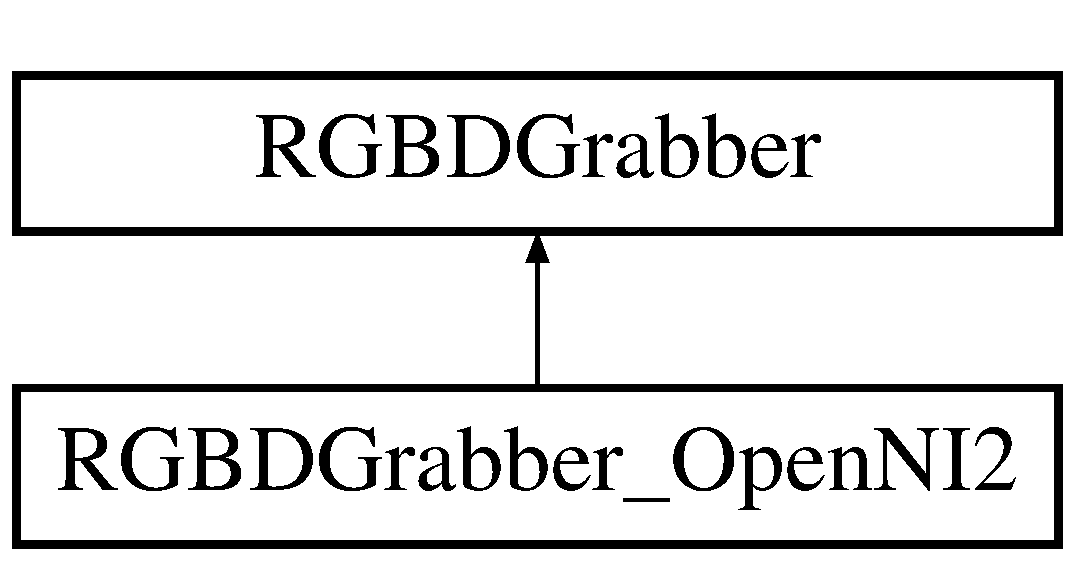
\includegraphics[height=2.000000cm]{classRGBDGrabber}
\end{center}
\end{figure}
\subsection*{Public Member Functions}
\begin{DoxyCompactItemize}
\item 
virtual void \hyperlink{classRGBDGrabber_ad4f514ef7ef4cb30f88691576cd2a415}{init} ()=0
\item 
virtual void \hyperlink{classRGBDGrabber_a5421d2f64b001189aaddb517bd50f973}{grab} (Frame\-R\-G\-B\-D $\ast$)=0
\item 
virtual void \hyperlink{classRGBDGrabber_aa835859ea230e1ca302adaa4cb054207}{stop} ()=0
\end{DoxyCompactItemize}
\subsection*{Protected Attributes}
\begin{DoxyCompactItemize}
\item 
int \hyperlink{classRGBDGrabber_aafd74a114077376b2326476e1b65ce20}{width}
\item 
\hypertarget{classRGBDGrabber_a5b03f2b35c58d70db79db90728558f7f}{int {\bfseries height}}\label{classRGBDGrabber_a5b03f2b35c58d70db79db90728558f7f}

\item 
cv\-::\-Mat \hyperlink{classRGBDGrabber_a077f46c80736207093874e307e53b269}{current\-R\-G\-B\-Img}
\item 
\hypertarget{classRGBDGrabber_a942fbb8ab02ac4d30fef4dadd20a0e7c}{cv\-::\-Mat {\bfseries current\-Depth\-Img}}\label{classRGBDGrabber_a942fbb8ab02ac4d30fef4dadd20a0e7c}

\end{DoxyCompactItemize}


\subsection{Detailed Description}
Abstract class that especifies the functionality of a generic R\-G\-B\-D grabber. 

\subsection{Member Function Documentation}
\hypertarget{classRGBDGrabber_a5421d2f64b001189aaddb517bd50f973}{\index{R\-G\-B\-D\-Grabber@{R\-G\-B\-D\-Grabber}!grab@{grab}}
\index{grab@{grab}!RGBDGrabber@{R\-G\-B\-D\-Grabber}}
\subsubsection[{grab}]{\setlength{\rightskip}{0pt plus 5cm}virtual void R\-G\-B\-D\-Grabber\-::grab (
\begin{DoxyParamCaption}
\item[{Frame\-R\-G\-B\-D $\ast$}]{}
\end{DoxyParamCaption}
)\hspace{0.3cm}{\ttfamily [pure virtual]}}}\label{classRGBDGrabber_a5421d2f64b001189aaddb517bd50f973}
Retains the current R\-G\-B\-D frame. 

Implemented in \hyperlink{classRGBDGrabber__OpenNI2_affad3812ddfff63085e03a30686db3ac}{R\-G\-B\-D\-Grabber\-\_\-\-Open\-N\-I2}.

\hypertarget{classRGBDGrabber_ad4f514ef7ef4cb30f88691576cd2a415}{\index{R\-G\-B\-D\-Grabber@{R\-G\-B\-D\-Grabber}!init@{init}}
\index{init@{init}!RGBDGrabber@{R\-G\-B\-D\-Grabber}}
\subsubsection[{init}]{\setlength{\rightskip}{0pt plus 5cm}virtual void R\-G\-B\-D\-Grabber\-::init (
\begin{DoxyParamCaption}
{}
\end{DoxyParamCaption}
)\hspace{0.3cm}{\ttfamily [pure virtual]}}}\label{classRGBDGrabber_ad4f514ef7ef4cb30f88691576cd2a415}
Initializes the grabber object 

Implemented in \hyperlink{classRGBDGrabber__OpenNI2_afbf7a0c2b858bad4d660104386073bb8}{R\-G\-B\-D\-Grabber\-\_\-\-Open\-N\-I2}.

\hypertarget{classRGBDGrabber_aa835859ea230e1ca302adaa4cb054207}{\index{R\-G\-B\-D\-Grabber@{R\-G\-B\-D\-Grabber}!stop@{stop}}
\index{stop@{stop}!RGBDGrabber@{R\-G\-B\-D\-Grabber}}
\subsubsection[{stop}]{\setlength{\rightskip}{0pt plus 5cm}virtual void R\-G\-B\-D\-Grabber\-::stop (
\begin{DoxyParamCaption}
{}
\end{DoxyParamCaption}
)\hspace{0.3cm}{\ttfamily [pure virtual]}}}\label{classRGBDGrabber_aa835859ea230e1ca302adaa4cb054207}
Stop grabing R\-G\-B\-D frames. 

Implemented in \hyperlink{classRGBDGrabber__OpenNI2_af986000241075e4e7cc0343b391d2eb6}{R\-G\-B\-D\-Grabber\-\_\-\-Open\-N\-I2}.



\subsection{Member Data Documentation}
\hypertarget{classRGBDGrabber_a077f46c80736207093874e307e53b269}{\index{R\-G\-B\-D\-Grabber@{R\-G\-B\-D\-Grabber}!current\-R\-G\-B\-Img@{current\-R\-G\-B\-Img}}
\index{current\-R\-G\-B\-Img@{current\-R\-G\-B\-Img}!RGBDGrabber@{R\-G\-B\-D\-Grabber}}
\subsubsection[{current\-R\-G\-B\-Img}]{\setlength{\rightskip}{0pt plus 5cm}cv\-::\-Mat R\-G\-B\-D\-Grabber\-::current\-R\-G\-B\-Img\hspace{0.3cm}{\ttfamily [protected]}}}\label{classRGBDGrabber_a077f46c80736207093874e307e53b269}
Resolution mode of the device (default is Q\-V\-G\-A = 320x240) \hypertarget{classRGBDGrabber_aafd74a114077376b2326476e1b65ce20}{\index{R\-G\-B\-D\-Grabber@{R\-G\-B\-D\-Grabber}!width@{width}}
\index{width@{width}!RGBDGrabber@{R\-G\-B\-D\-Grabber}}
\subsubsection[{width}]{\setlength{\rightskip}{0pt plus 5cm}int R\-G\-B\-D\-Grabber\-::width\hspace{0.3cm}{\ttfamily [protected]}}}\label{classRGBDGrabber_aafd74a114077376b2326476e1b65ce20}
Frame dimensions. 

The documentation for this class was generated from the following file\-:\begin{DoxyCompactItemize}
\item 
grabber/R\-G\-B\-D\-Grabber.\-h\end{DoxyCompactItemize}

\hypertarget{classRGBDGrabber__OpenNI2}{\section{R\-G\-B\-D\-Grabber\-\_\-\-Open\-N\-I2 Class Reference}
\label{classRGBDGrabber__OpenNI2}\index{R\-G\-B\-D\-Grabber\-\_\-\-Open\-N\-I2@{R\-G\-B\-D\-Grabber\-\_\-\-Open\-N\-I2}}
}


{\ttfamily \#include $<$R\-G\-B\-D\-Grabber\-\_\-\-Open\-N\-I2.\-h$>$}

Inheritance diagram for R\-G\-B\-D\-Grabber\-\_\-\-Open\-N\-I2\-:\begin{figure}[H]
\begin{center}
\leavevmode
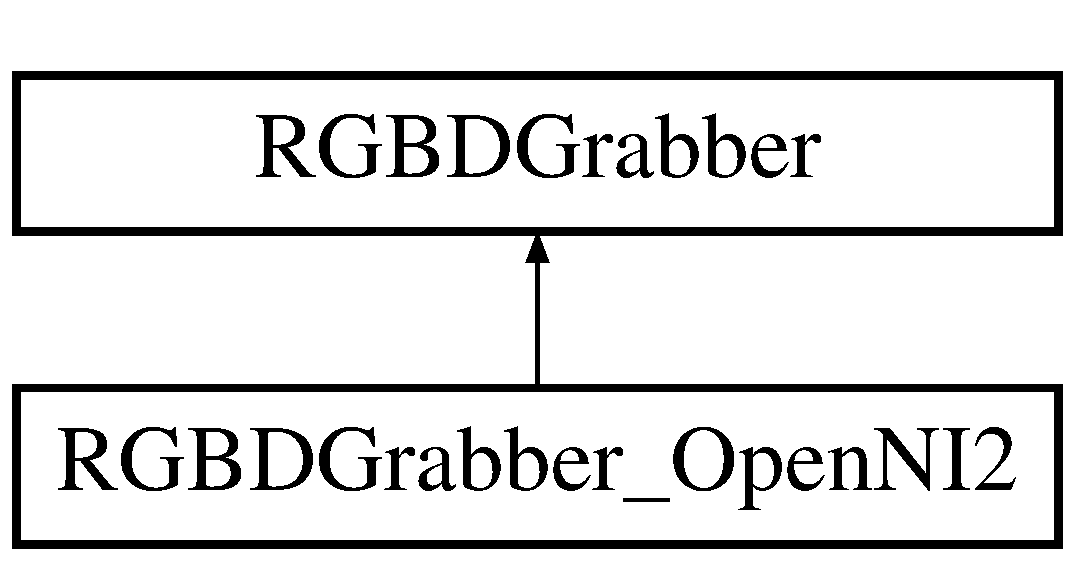
\includegraphics[height=2.000000cm]{classRGBDGrabber__OpenNI2}
\end{center}
\end{figure}
\subsection*{Public Member Functions}
\begin{DoxyCompactItemize}
\item 
\hyperlink{classRGBDGrabber__OpenNI2_ab345f03078f20ffb30edccbf2ef70892}{R\-G\-B\-D\-Grabber\-\_\-\-Open\-N\-I2} (const char $\ast$uri=openni\-::\-A\-N\-Y\-\_\-\-D\-E\-V\-I\-C\-E, const int mode=1)
\item 
void \hyperlink{classRGBDGrabber__OpenNI2_aaf62639ea4a14acac0fee7e11fdc5bf9}{show\-Available\-Modes} ()
\item 
void \hyperlink{classRGBDGrabber__OpenNI2_a6d6ba5b908bcdf8442bd083958b38036}{set\-Resolution} (int res)
\item 
void \hyperlink{classRGBDGrabber__OpenNI2_aeebcaa5079629654dc30f0fdbaacea61}{set\-Shutter} (int exposure)
\item 
int \hyperlink{classRGBDGrabber__OpenNI2_a68dc63b53be20c9feecbb7d78c5121c3}{get\-Shutter} ()
\item 
void \hyperlink{classRGBDGrabber__OpenNI2_a7a3d58b840b8c6b049bb8aa5e043e935}{set\-Gain} (int gain)
\item 
int \hyperlink{classRGBDGrabber__OpenNI2_a3e3e079f580c988ec37369ab1a468c1c}{get\-Gain} ()
\item 
void \hyperlink{classRGBDGrabber__OpenNI2_afbf7a0c2b858bad4d660104386073bb8}{init} ()
\item 
void \hyperlink{classRGBDGrabber__OpenNI2_affad3812ddfff63085e03a30686db3ac}{grab} (Frame\-R\-G\-B\-D $\ast$frame\-Ptr)
\item 
void \hyperlink{classRGBDGrabber__OpenNI2_af986000241075e4e7cc0343b391d2eb6}{stop} ()
\end{DoxyCompactItemize}
\subsection*{Additional Inherited Members}


\subsection{Detailed Description}
This class captures R\-G\-B\-D frames from an Open\-N\-I2 compatible sensor. It grabs the intensity and depth images and stores them in a 'Frame\-R\-G\-B\-D' object. 

\subsection{Constructor \& Destructor Documentation}
\hypertarget{classRGBDGrabber__OpenNI2_ab345f03078f20ffb30edccbf2ef70892}{\index{R\-G\-B\-D\-Grabber\-\_\-\-Open\-N\-I2@{R\-G\-B\-D\-Grabber\-\_\-\-Open\-N\-I2}!R\-G\-B\-D\-Grabber\-\_\-\-Open\-N\-I2@{R\-G\-B\-D\-Grabber\-\_\-\-Open\-N\-I2}}
\index{R\-G\-B\-D\-Grabber\-\_\-\-Open\-N\-I2@{R\-G\-B\-D\-Grabber\-\_\-\-Open\-N\-I2}!RGBDGrabber_OpenNI2@{R\-G\-B\-D\-Grabber\-\_\-\-Open\-N\-I2}}
\subsubsection[{R\-G\-B\-D\-Grabber\-\_\-\-Open\-N\-I2}]{\setlength{\rightskip}{0pt plus 5cm}R\-G\-B\-D\-Grabber\-\_\-\-Open\-N\-I2\-::\-R\-G\-B\-D\-Grabber\-\_\-\-Open\-N\-I2 (
\begin{DoxyParamCaption}
\item[{const char $\ast$}]{uri = {\ttfamily openni\-:\-:ANY\-\_\-DEVICE}, }
\item[{const int}]{mode = {\ttfamily 1}}
\end{DoxyParamCaption}
)\hspace{0.3cm}{\ttfamily [inline]}}}\label{classRGBDGrabber__OpenNI2_ab345f03078f20ffb30edccbf2ef70892}
Connected devices information

Constructor. Creates a \hyperlink{classRGBDGrabber__OpenNI2}{R\-G\-B\-D\-Grabber\-\_\-\-Open\-N\-I2} instance that grabs R\-G\-B\-D frames from an Open\-N\-I compatible sensor. 

\subsection{Member Function Documentation}
\hypertarget{classRGBDGrabber__OpenNI2_a3e3e079f580c988ec37369ab1a468c1c}{\index{R\-G\-B\-D\-Grabber\-\_\-\-Open\-N\-I2@{R\-G\-B\-D\-Grabber\-\_\-\-Open\-N\-I2}!get\-Gain@{get\-Gain}}
\index{get\-Gain@{get\-Gain}!RGBDGrabber_OpenNI2@{R\-G\-B\-D\-Grabber\-\_\-\-Open\-N\-I2}}
\subsubsection[{get\-Gain}]{\setlength{\rightskip}{0pt plus 5cm}int R\-G\-B\-D\-Grabber\-\_\-\-Open\-N\-I2\-::get\-Gain (
\begin{DoxyParamCaption}
{}
\end{DoxyParamCaption}
)\hspace{0.3cm}{\ttfamily [inline]}}}\label{classRGBDGrabber__OpenNI2_a3e3e079f580c988ec37369ab1a468c1c}
Return the current Gain value (in percentage 100\%). \hypertarget{classRGBDGrabber__OpenNI2_a68dc63b53be20c9feecbb7d78c5121c3}{\index{R\-G\-B\-D\-Grabber\-\_\-\-Open\-N\-I2@{R\-G\-B\-D\-Grabber\-\_\-\-Open\-N\-I2}!get\-Shutter@{get\-Shutter}}
\index{get\-Shutter@{get\-Shutter}!RGBDGrabber_OpenNI2@{R\-G\-B\-D\-Grabber\-\_\-\-Open\-N\-I2}}
\subsubsection[{get\-Shutter}]{\setlength{\rightskip}{0pt plus 5cm}int R\-G\-B\-D\-Grabber\-\_\-\-Open\-N\-I2\-::get\-Shutter (
\begin{DoxyParamCaption}
{}
\end{DoxyParamCaption}
)\hspace{0.3cm}{\ttfamily [inline]}}}\label{classRGBDGrabber__OpenNI2_a68dc63b53be20c9feecbb7d78c5121c3}
Return the current Exposure value (in milliseconds). \hypertarget{classRGBDGrabber__OpenNI2_affad3812ddfff63085e03a30686db3ac}{\index{R\-G\-B\-D\-Grabber\-\_\-\-Open\-N\-I2@{R\-G\-B\-D\-Grabber\-\_\-\-Open\-N\-I2}!grab@{grab}}
\index{grab@{grab}!RGBDGrabber_OpenNI2@{R\-G\-B\-D\-Grabber\-\_\-\-Open\-N\-I2}}
\subsubsection[{grab}]{\setlength{\rightskip}{0pt plus 5cm}void R\-G\-B\-D\-Grabber\-\_\-\-Open\-N\-I2\-::grab (
\begin{DoxyParamCaption}
\item[{Frame\-R\-G\-B\-D $\ast$}]{frame\-Ptr}
\end{DoxyParamCaption}
)\hspace{0.3cm}{\ttfamily [inline]}, {\ttfamily [virtual]}}}\label{classRGBDGrabber__OpenNI2_affad3812ddfff63085e03a30686db3ac}
Copy the current R\-G\-B\-D frame into 'frame\-Ptr'. 

Implements \hyperlink{classRGBDGrabber_a5421d2f64b001189aaddb517bd50f973}{R\-G\-B\-D\-Grabber}.

\hypertarget{classRGBDGrabber__OpenNI2_afbf7a0c2b858bad4d660104386073bb8}{\index{R\-G\-B\-D\-Grabber\-\_\-\-Open\-N\-I2@{R\-G\-B\-D\-Grabber\-\_\-\-Open\-N\-I2}!init@{init}}
\index{init@{init}!RGBDGrabber_OpenNI2@{R\-G\-B\-D\-Grabber\-\_\-\-Open\-N\-I2}}
\subsubsection[{init}]{\setlength{\rightskip}{0pt plus 5cm}void R\-G\-B\-D\-Grabber\-\_\-\-Open\-N\-I2\-::init (
\begin{DoxyParamCaption}
{}
\end{DoxyParamCaption}
)\hspace{0.3cm}{\ttfamily [inline]}, {\ttfamily [virtual]}}}\label{classRGBDGrabber__OpenNI2_afbf7a0c2b858bad4d660104386073bb8}
Initializes the grabber object 

Implements \hyperlink{classRGBDGrabber_ad4f514ef7ef4cb30f88691576cd2a415}{R\-G\-B\-D\-Grabber}.

\hypertarget{classRGBDGrabber__OpenNI2_a7a3d58b840b8c6b049bb8aa5e043e935}{\index{R\-G\-B\-D\-Grabber\-\_\-\-Open\-N\-I2@{R\-G\-B\-D\-Grabber\-\_\-\-Open\-N\-I2}!set\-Gain@{set\-Gain}}
\index{set\-Gain@{set\-Gain}!RGBDGrabber_OpenNI2@{R\-G\-B\-D\-Grabber\-\_\-\-Open\-N\-I2}}
\subsubsection[{set\-Gain}]{\setlength{\rightskip}{0pt plus 5cm}void R\-G\-B\-D\-Grabber\-\_\-\-Open\-N\-I2\-::set\-Gain (
\begin{DoxyParamCaption}
\item[{int}]{gain}
\end{DoxyParamCaption}
)\hspace{0.3cm}{\ttfamily [inline]}}}\label{classRGBDGrabber__OpenNI2_a7a3d58b840b8c6b049bb8aa5e043e935}
Set the exposure value (in milliseconds). \hypertarget{classRGBDGrabber__OpenNI2_a6d6ba5b908bcdf8442bd083958b38036}{\index{R\-G\-B\-D\-Grabber\-\_\-\-Open\-N\-I2@{R\-G\-B\-D\-Grabber\-\_\-\-Open\-N\-I2}!set\-Resolution@{set\-Resolution}}
\index{set\-Resolution@{set\-Resolution}!RGBDGrabber_OpenNI2@{R\-G\-B\-D\-Grabber\-\_\-\-Open\-N\-I2}}
\subsubsection[{set\-Resolution}]{\setlength{\rightskip}{0pt plus 5cm}void R\-G\-B\-D\-Grabber\-\_\-\-Open\-N\-I2\-::set\-Resolution (
\begin{DoxyParamCaption}
\item[{int}]{res}
\end{DoxyParamCaption}
)\hspace{0.3cm}{\ttfamily [inline]}}}\label{classRGBDGrabber__OpenNI2_a6d6ba5b908bcdf8442bd083958b38036}
Set the resolution. \hypertarget{classRGBDGrabber__OpenNI2_aeebcaa5079629654dc30f0fdbaacea61}{\index{R\-G\-B\-D\-Grabber\-\_\-\-Open\-N\-I2@{R\-G\-B\-D\-Grabber\-\_\-\-Open\-N\-I2}!set\-Shutter@{set\-Shutter}}
\index{set\-Shutter@{set\-Shutter}!RGBDGrabber_OpenNI2@{R\-G\-B\-D\-Grabber\-\_\-\-Open\-N\-I2}}
\subsubsection[{set\-Shutter}]{\setlength{\rightskip}{0pt plus 5cm}void R\-G\-B\-D\-Grabber\-\_\-\-Open\-N\-I2\-::set\-Shutter (
\begin{DoxyParamCaption}
\item[{int}]{exposure}
\end{DoxyParamCaption}
)\hspace{0.3cm}{\ttfamily [inline]}}}\label{classRGBDGrabber__OpenNI2_aeebcaa5079629654dc30f0fdbaacea61}
Set the exposure value (in milliseconds). \hypertarget{classRGBDGrabber__OpenNI2_aaf62639ea4a14acac0fee7e11fdc5bf9}{\index{R\-G\-B\-D\-Grabber\-\_\-\-Open\-N\-I2@{R\-G\-B\-D\-Grabber\-\_\-\-Open\-N\-I2}!show\-Available\-Modes@{show\-Available\-Modes}}
\index{show\-Available\-Modes@{show\-Available\-Modes}!RGBDGrabber_OpenNI2@{R\-G\-B\-D\-Grabber\-\_\-\-Open\-N\-I2}}
\subsubsection[{show\-Available\-Modes}]{\setlength{\rightskip}{0pt plus 5cm}void R\-G\-B\-D\-Grabber\-\_\-\-Open\-N\-I2\-::show\-Available\-Modes (
\begin{DoxyParamCaption}
{}
\end{DoxyParamCaption}
)\hspace{0.3cm}{\ttfamily [inline]}}}\label{classRGBDGrabber__OpenNI2_aaf62639ea4a14acac0fee7e11fdc5bf9}
Shows a list of connected sensors

Set the sensor U\-R\-I.

Shows a list of the available modes for the chosen \hypertarget{classRGBDGrabber__OpenNI2_af986000241075e4e7cc0343b391d2eb6}{\index{R\-G\-B\-D\-Grabber\-\_\-\-Open\-N\-I2@{R\-G\-B\-D\-Grabber\-\_\-\-Open\-N\-I2}!stop@{stop}}
\index{stop@{stop}!RGBDGrabber_OpenNI2@{R\-G\-B\-D\-Grabber\-\_\-\-Open\-N\-I2}}
\subsubsection[{stop}]{\setlength{\rightskip}{0pt plus 5cm}void R\-G\-B\-D\-Grabber\-\_\-\-Open\-N\-I2\-::stop (
\begin{DoxyParamCaption}
{}
\end{DoxyParamCaption}
)\hspace{0.3cm}{\ttfamily [inline]}, {\ttfamily [virtual]}}}\label{classRGBDGrabber__OpenNI2_af986000241075e4e7cc0343b391d2eb6}
Stop grabing R\-G\-B\-D frames. 

Implements \hyperlink{classRGBDGrabber_aa835859ea230e1ca302adaa4cb054207}{R\-G\-B\-D\-Grabber}.



The documentation for this class was generated from the following file\-:\begin{DoxyCompactItemize}
\item 
grabber/R\-G\-B\-D\-Grabber\-\_\-\-Open\-N\-I2.\-h\end{DoxyCompactItemize}

\addcontentsline{toc}{part}{Index}
\printindex
\end{document}
